\chapter{Testing}

\section{Overall Approach to Testing}
Overall approach to testing was fairly simple, with the completion of each feature any relevant tests were either coded or completed by the developer. This included unit testing, stress testing and acceptance testing. Due to the applications aim of helping a user it was important the UI was received well. 
\subsection{Problems Encountered}
Throughout testing many issues arose, many more than were found in development. Getting a working test environment functional for the first time was much more complicated than expected, with references to this around the web it is not an isolated incident. Problems included - 
\begin{itemize}
  \item Out of date documentation on the official Google Developer site.
  \item Bugs in the current (1.2) version of Android Studio which will show an empty test suite despite the tests being there, ran and results printed.
  \item Lack of official support for unit testing in Activity classes, while it seems possible the issues it proves are numerous. Alternatives were discovered near the end of the project time line but a lack of time meant other more important tasks were completed.  
\end{itemize}

In future projects more time will have to be dedicated to the testing of the application. It is thought the issues encountered with testing were down to mix of issues, mainly the early stages of Android Studios official release and the tight schedule for testing including final acceptance testing. 
\section{Automated Testing}
Automated testing was completed throughout the duration of the project, problems with unit testing were previously discussed however Android did have other important utilities to make use of which helped with thorough testing, especially looking for crash cases.
\subsection{Unit Tests}
Despite the issues encountered, unit testing was completed on the non Activity classes. This included the testing of correct behaviour from the classes to handle distance calculations and from the Objects which made up a Route Object. While the tests results would not appear within the IDE due to a known bug it was still possible to see the results in a created HTML document logging pass percentage. While it would have been beneficial to complete more Unit testing it would have required the re structuring of the program and reversal of many design decisions. While an attempt to follow a MVP pattern was made, as can be seen with the XML, Route Display Activity and Route object, in future it is advised it is stuck to more thoroughly to aid with testing. 

\begin{figure}[H]
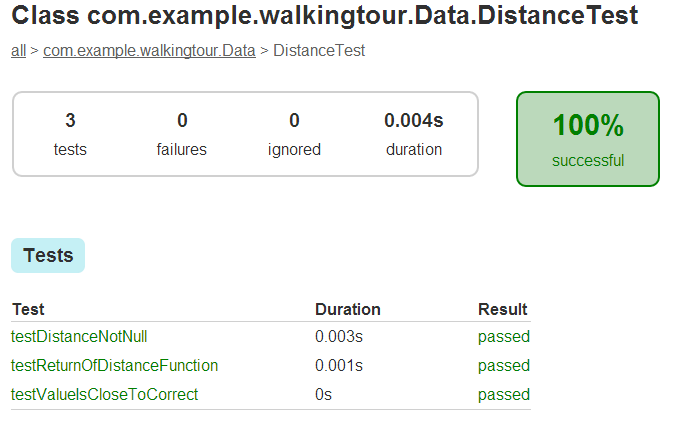
\includegraphics[scale=0.5]{Chapter4/unit.png} 
\caption[Test Output]{Image displaying the output from running a set of tests, these are results from a single small set of tests.}
\end{figure}
\subsection{Stress Testing}
Stress testing was completed with the use of 'The Monkey'. 'The Monkey' is a tool which sends a range of inputs to the application and logs the results of this at the end of its run. By doing this the application is spammed with events and any area of the application where hang ups in performance can cause crashes should be found. Through final stress testing well over 200,000 inputs have been simulated and no serious faults can be found in the application. However this does not mean that faults are not there, just hard to find if they are. 

Throughout stress testing one issue which has been prevalent however has been the lack of support for the cancelling of activities, this has been noted in both the route data entry screen and the route choice screen. Since then these have been handled along with the addition of further tests in the code to deal with a user selecting the same location as a start and destination. 

Using 'The Monkey' tool was a real benefit for the developer, as pointed out while it found no significant errors the ones it did find would have caused a real effect on the usability of the application. In future it is advised any improvement to the application be tested in such a way, the tool can be limited to the use of a single package and as such can be fine tuned to send demands to the right class. 

\begin{figure}[H]
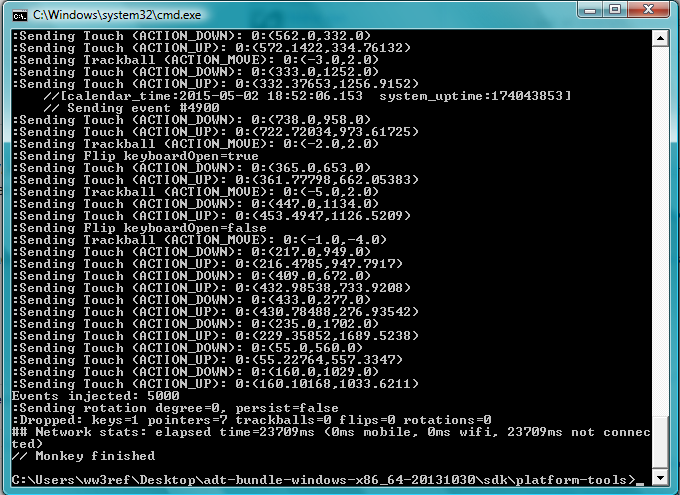
\includegraphics[scale=0.5]{Chapter4/monkey.png} 
\caption[Monkey Stress Test]{Image displaying the results of a Monkey run using 5000 inputs resulting in no dropped actions and no crashes on the device side.}
\end{figure}

\section{Integration Testing}
While some integration testing was completed there is little to document due to the nature of the application. This is down to the fact that the functionality within the application are essentially singular branches accessed through the Menu Activity. As this is the structure, very little is passed between multiple functionalities, the only place this can be seen is the file from the Route Plotter being compatible with the Route Finder graph structure. So while testing was completed, the initial unit testing combined with final acceptance testing was seen as sufficient.
\section{User Testing}
After initial development a small user group was used to determine some UI elements, this mainly related to the use of the application for first time users and the overall visual appeal of the application. For these tests users were asked to perform a variety of tasks relating to the functional requirements, the results of these can be seen in the Appendix section C. Users were also asked for their opinion on the colour scheme of the application, this was done through the use of different themes for different pages on the test application. While some of the features were a little bare at the time they were all fully functional, just not polished. Results from these tests were used to set the theme however little was discovered from the small user group. In future it is advised a much larger group is used.
\section{Acceptance Testing}
Acceptance Testing was performed by the developer of the application, a list of tests was drawn up to determine the full functionality of the application including cases which may cause crashes from poor quality code. The test tables which represent this information can be found in Appendix section C. Some were completed after full development, others during development.
\section{Testing Evaluation}
While the developer feels a sufficient amount of testing was completed for the time given, it is still lacking in terms of a full project. Ideally a whole restructuring of the program should be undertaken to help with unit testing and a better adherence to the MVP pattern which is ideal for this situation and Android in general. 